\section{x-commerce design}
\label{sec:document_driven_web_development_process}
At the design stage, we have identified two solutions for the management of the resources used by the client and by the administrator of x-commerce. In particular, the client of x-commerce have different needs in the use of the platform than the administrator. While the former is more oriented to the use of the information on products and eventually to the order, the administrator is more concerned with the inclusion of new products and information in order to better organize the resources and the interface offered to the customer. Considering that the two main actors involved in these interactions require different levels of security. Only the administrator can modify the information and all other eligible data.
\newline
To separate this client management and administrator e-commerce, it was decided to separate the pages of the administrator and client in two different directories. This allows you to host the administrator on a server other than the server on which the client access to x-commerce. This does not however exclude the possibility of offering two types of services from a single server.
\newline
This organization of pages for the client and the administrator allows you to assign the same name to the pages and its parts.
\newline
The process to build a web application based on x-commerce toolkit consists of the following four steps: defining the model of the schema, HTTP RESTful API definition, UI components definition and assembly.
\subsection{Model schemas definition}
A description of entities, properties, relations and data access policies are defined as JSON documents.
\newline
The models of e-commerce are many and are expected to grow further with the integration and implementation of new services. At the moment there are 30 models. Loopback in the definition of each model is done by filling in a JSON file where declare properties that interest us. In the following are the main models of x-commerce:
\begin{itemize}
\item \emph{product}: the model has many properties, but we are specifying the properties which are of greater interest; for which:
\begin{itemize}
\item a product has a title string (we are also saying that this field is required);
\item a product has a description string;
\item a product has a price of type Number, etc..
\end{itemize}
The model has also produced the “relations”. This field identifies relation of the current model (“product”) with other models such as:
\begin{itemize}
\item a product has a relationship with the model “Image” type “many”. This report was modeled because the product has a lot of pictures;
\item a product has the relationship with the model “Comments” type “many” because a product has many comments or reviews, etc.
\item it is possible also to specify “acls (access control lists)” to control access to the system. Thus by specifying who can do what with a JSON file, it is possible to have a transparent way all security mechanisms.
\end{itemize}
\begin{lstlisting}[language=json]
{
  "name": "Product",
  "properties": {
    "title": { "type": "String", "required": true },
    "description": { "type": "String" },
    "price":  { "type": "Number" },
  },
  "relations": {
    "images": { "type": "hasMany", "model": "Image" },
    "comments": { "type": "hasMany", "model": "Comment" },
    "collections": { "type": "hasAndBelongsToMany", "model": "Collection" },
    "options": { "type": "hasMany", "model": "ProductOption" },
    "product_type": { "type": "belongsTo", "model": "ProductType" },
    "variants": { "type": "hasMany", "model": "ProductVariant" },
    "vendor": { "type": "belongsTo", "model": "Vendor"}
  }
}
\end{lstlisting}
\item \emph{customers}: this time there are two new things:
\begin{itemize}
\item the presence of \emph{acls}: in this case acls block all calls except “find” and count” that can call all;
\item note the presence of the \emph{“base”: “Users”}: “Users” is a model of loopback that is offered for free. This model brings back all funtionality related to login, sign up, forgot etc. “Customer” model extends the “Users” loopback, and in this way the “Customer” legacy capabilities and therefore all methods APIs and “Users” including methods for login and logout.
\begin{lstlisting}[language=json]
{
  "name": "Customer",
  "base": "User",
  "properties": {
    "first_name": { "type": "String", "required": true },
    "last_name": { "type": "String", "required": true },
    "date_of_birth" : { "type": "Date" },
    "gender": { "type": "String", "enum": ["M", "F"] },
    "email": { "type": "String", "required": true }
  }
}
\end{lstlisting}
\end{itemize}
\end{itemize}

Each JSON file is also accompanied by a js file. This file is used to define the so-called “hooks” or the methods to define new APIs customized. These new APIs are added to the API generated by the JSON file.
\begin{lstlisting}[language=javascript]
module.exports = function (Product) {
};
\end{lstlisting}
Inside the function offered to extend the API, it is possbile to define new APIs. The name of the API is declared as follows:
\begin{lstlisting}[language=javascript]
module.exports = function (Product) {
  Product.remoteMethod('generate_variants', {
    accepts: { arg: 'product_id', type: 'string', required: true },
    returns: { arg: 'variants', type: 'Array' },
    http: { verb: 'get', path:'/generate”' }
  });
};
\end{lstlisting}
The remote method takes two parameters:
\begin{itemize}
\item the name of the method to execute the call of the API in question. In this way, the method name is “generate\_variants”. This method will be executed when it is called api: “/api/Products/generate”;
\item as the second parameter, the remote method accepts a JSON object consisting of key-value pairs:
\begin{itemize}
\item “accepts”: indicates the input parameters that is, parameters that are present in the body of the request. In this case the input parameter is the only one and is of type String and is required.
\item “returns”: It indicates what type is the response;
\item “http”: This is a parameter that defines url API. Therefore, url for calling the generate API is: “/api/Products/generate”. When you call this API, it is invoked and executed the remote method declared as the first parameter. The remote method must be defined freely by the programmer.
\end{itemize}
\end{itemize}
Therefore, the complete example to define new APIs via remote methods, which are not generated by default from JSON file, is the following:
\begin{lstlisting}[language=javascript]
module.exports = function (Product) {
  Product.generate_variants = function (product_id, callback) {
    // to do anythings. Genreate a result
    callback(null, result);
  };

  Product.remoteMethod('generate_variants', {
    accepts: { arg: 'product_id', type: 'string', required: true },
    returns: { arg: 'variants', type: 'Array' },
    http: { verb: 'get', path:'/generate' }
  });
};
\end{lstlisting}
\subsection{HTTP RESTful API definition}
CRUD operations on models which are automatically generated by the web framework (on the basis of input JSON documents) and further custom actions can be defined. Following models of e-commerce are:
\begin{itemize}
\item \emph{products}: as already mentioned, it is the main model of the project. The properties of this model are easy to imagine because to buy a product, the most searched item is its properties. So a product has:
\begin{itemize}
\item \emph{title}: type string;
\item \emph{description}: type string;
\item \emph{price}: type Number;
\item \emph{compare\_at\_price}: type Number - This data is related to the “free” product and is used to show a reduced price to the client-side;
\item \emph{is\_charge\_taxes}: type Boolean - This data is used to load the order of taxes or not. Some customers may be absent from paying taxes;
\item \emph{sku}: type String - stock keeping unit or SKU - is a number or string of alpha and numeric characters that uniquely identify a product;
\item \emph{barcode}: type String - is the small image of lines (bars) and spaces that is affixed to retail store items, identification cards, and postal mail to identify a particular product number, person, or location;
\item \emph{track\_quantity}: type Boolean - used to keep track of the amount of products.
\item \emph{quantity}: type Number;
\item \emph{sell\_after\_purchase}: type Boolean;
\item \emph{unit\_measure\_weight}: type String;
\item \emph{weight}: type Number;
\item \emph{is\_published}: type Boolean;
\item \emph{published\_at}: type Date;
\item \emph{tags}: type Array of String
\end{itemize}
\item \emph{article}: this model is used to represent items or news to add to the blog of x-commerce.
\begin{lstlisting}[language=json]
{
  "name": "Article",
  "properties": {
    "title": { "type": "string", "required": true },
    "subtitle": { "type": "string" },
    "summary": { "type": "string" },
    "content": { "type": "string" },
    "created_at": { "type": "date" },
    "updated_at": { "type": "date" },
    "published_at": { "type": "date" },
    "tags": { "type": ["string"] }
  },
  "relations": {
    "author": { "type": "belongsTo", "model": "Manager" },
    "category": { "type": "belongsTo", "model": "Category" },
    "images": { "type": "hasMany", "model": "Image" }
  }
}
\end{lstlisting}
\item \emph{collections}: this model is used to represent collections, for example: summer, winter, spring, autumn. A product may belong to one or more collections.
\begin{lstlisting}[language=json]
{
  "name": "Collection",
  "properties": {
    "title": { "type": "String", "required": true },
    "description": { "type": "String" },
    "is_published": { "type": "Boolean" },
    "published_at": { "type": "Date" }
  },
  "relations": {
    "images": { "type": "hasMany", "model": "Image" },
    "products": { "type": "hasAndBelongsToMany", "model": "Product"}
  }
}
\end{lstlisting}
\item \emph{comments}: this model is used to represent customer reviews.
\begin{lstlisting}
{
  "name": "Comment",
  "properties": {
    "title": { "type": "String" },
    "text": { "type": "String" },
    "created_at": { "type": "Date" }
  },
  "relations": {
    "author": { "type": "belongsTo", "model": "Customer" },
    "replies": { "type": "hasMany", "model": "CommentReply" }
  }
}
\end{lstlisting}
\item \emph{coupons}: this model is used to represent the coupons. The admin can generate insert, delete new coupon.
\begin{lstlisting}
{
  "name": "Coupon",
  "properties": {
    "name": { "type": "String", "required": true },
    "description": { "type": "String" },
    "discount": { "type": "Number", "required": true },
    "code": { "type": "String", "required": true },
    "date_from": { "type": "Date" },
    "date_to": { "type": "Date" }
  },
  "relations": {
    "order": { "type": "belongsTo", "model": "Order" }
  }
}
\end{lstlisting}
\item \emph{images}: A product, collectione etc can have one or more images. This model is for storing image information.
\begin{lstlisting}
{
  "name": "Image",
  "properties": {
    "thumbs": { "type": "array" },
    "description": { "type": "string" },
    "filename": { "type": "string" }
  }
}
\end{lstlisting}
\item \emph{orders}: The model order is one of the main models of e-commerce that is used to model an order. An order consists of more lines and order belongs to a customer.
\begin{lstlisting}
{
  "name": "Order",
  "properties": {
    "status": { "type": "String", "default": "open",
      "enum": ["open", "pending", "paid", "closed"],
      "required": true },
    "discount": { "type": "Number" },
    "shipping_cost": { "type": "Number" },
    "taxes": { "type": "Number" },
    "total": { "type": "Number" }
  },
  "relations": {
    "customer": { "type": "belongsTo", "model": "Customer" },
    "order_items": { "type": "hasMany", "model": "OrderItem" },
    "payments": { "type": "hasMany", "model": "Payment" },
    "taxes": { "type": "hasMany", "model": "Tax" }
  }
}
\end{lstlisting}
\item \emph{order\_items}: an Order has more lines of order and therefore has a relationship with the model OrderItems used to represent information in a single line command.
\begin{lstlisting}
{
  "name": "OrderItem",
  "properties": {
    "quantity": { "type": "Number" }
  },
  "relations": {
    "product": { "type": "belongsTo", "model": "Product" },
    "product_variant": { "type": "belongsTo", "model": "ProductVariant" }
  }
}
\end{lstlisting}
\item \emph{payments}: to store information relating to the payment has been used the model Payment.
\begin{lstlisting}
{
  "name": "Payment",
  "properties": {
    "payment_method": { "type": "String" },
    "payment": { "type": "Object" }
  }
}
\end{lstlisting}
\item \emph{product\_options}: a product can have the optional information such as a T-shirt may have different measures as: S, M, L, XL, etc .. In order to model this aspect was created ProductOption model.
\begin{lstlisting}
{
  "name": "ProductOption",
  "properties": {
    "name": { "type": "String" },
    "values": { "type": ["String"] },
    "type": { "type": "String" }
  }
}
\end{lstlisting}
\item \emph{product\_types}: a product may have special information that need to be represented as such as a shirt may be of: cotton, silk, etc...
To represent this peculiarity of a product is created ProductOption model.
\begin{lstlisting}
{
  "name": "ProductType",
  "properties": {
    "name": { "type": "String", "required": true },
    "description":{ "type": "String" }
  }
}
\end{lstlisting}
\item \emph{product\_variants}: the set of options a product represents a variant. It can be a shirt size L (option 1) and be red (option 2) etc...
The product showed the customer to x-commerce, it is also very variant \emph{L-red}.
\begin{lstlisting}
{
  "name": "ProductVariant",
  "properties": {
    "name": { "type": "String", "required": true },
    "combo": { "type": ["String"], "required": true },
    "price": { "type": "Number" },
    "sku": { "type": "String" },
    "barcode": { "type": "String" }
  },
  "relations": {
    "product": { "type": "belongsTo", "model": "Product" }
  }
}
\end{lstlisting}
\item \emph{stores}: this model is used to represent information about the store such as name, description, policy, phone, etc...
\begin{lstlisting}
{
  "name": "Store",
  "properties": {
    "name": { "type": "String", "default": "x-commerce", "required": true },
    "description": { "type": "String", "required": true },
    "mobile_phone": { "type": "String" },
    "office_phone": { "type": "String" },
    "email": { "type": "String", "length": 64, "required": true },
    "policy": { "type": "String" }
  },
  "relations": {
    "nexus": { "type": "belongsTo", "model": "Nexus" },
    "image": { "type": "hasOne", "model": "Image" }
  }
}
\end{lstlisting}
\item \emph{tasks}: payment or any operation can fail. In this case you need to store some information about the operation performed and then try again. The Task model therefore serves to store information to retry the operation.
\begin{lstlisting}
{
  "name": "Task",
  "properties": {
    "data": { "type": "Object" },
    "handler": { "type": "String" },
    "created_at": { "type": "Date" },
    "priority": { "type": "String", "default": "low",
    "enum": ["low", "medium", "high"] },
    "last_retry_at": { "type": "Date" },
    "retry_count": { "type": "Number" },
    "done_at": { "type": "Date" },
    "done": { "type": "Boolean" }
  }
}
\end{lstlisting}
\item \emph{taxes}: this model is used to store information on the fees payable related to an order.
\begin{lstlisting}
{
  "name": "Tax",
  "properties": {
    "name": { "type": "String" },
    "description": { "type": "String" },
    "reason":{ "type": "String" },
    "import": { "type": "Number" }
  }
}
\end{lstlisting}
\item \emph{vendors}: a product is inserted by a seller. To store information about the vendor, it was created the model Vendor.
\begin{lstlisting}
{
  "name": "Vendor",
  "properties": {
    "name": { "type": "String", "required": true },
    "description": { "type": "String" }
  }
}
\end{lstlisting}
\item \emph{wishlists}: in systems of e-commerce it is very important to give the client the possibility of costuire their wishlist. This is why you created Wishlist model.
\begin{lstlisting}
{
  "name": "Wishlist",
  "properties": {
    "product_id": { "type": "String" },
    "product_variant_id": { "type": "String" },
    "description": { "type": "String" }
  },
  "relations": {
    "product": { "type": "belongsTo", "model": "Product" },
    "product_variant": { "type": "belongsTo", "model": "ProductVariant" }
  }
}
\end{lstlisting}
\end{itemize}
All of them are exposed as HTTP RESTful API. APIs generated for the basic model Product:
\begin{itemize}
\item \textbf{POST /products} — Create a new instance of the model and persist it into the data source;
\item \textbf{GET /products} —  Find all instances of the model matched by filter from the data source;
\item \textbf{PUT /products} — Update an existing model instance or insert a new one into the data source;
\item \textbf{PUT /products/id} — Update attributes for a model instance and persist it into the data source;
\item \textbf{GET /products/id} — Find a model instance by id from the data source;
\item \textbf{DELETE /products/id} — Delete a model instance by id from the data source;
\item \textbf{GET  /products/count} — Count instances of the model matched by where from the data source;
\item \textbf{GET /products/findOne}  - Find first instance of the model matched by filter from the data source;
\item \textbf{POST /products/update} — Update instances of the model matched by where from that data source;
\item \textbf{GET /products/id/collections} — Queries collections of Product. A product has a relationship with collection type: hasAndBelongsToMany. Loopback then it generates all possible API to manage the relations. In this case it is shown only the GET;
\item \textbf{GET  /products/id/comments} — Queries comments of Product. A product has a relationship with Comment type: hasMany. Loopback then it generates all possible API to manage the relations. In this case it is shown only the GET;
\item \textbf{POST /products/id/images} — Queries images of Product. A product has a relationship with Image type: hasMany. Loopback then it generates all possible API to manage the relations. In this case it is shown only the GET;
\item \textbf{POST /products/id/options} — Queries options of Product. A product has a relationship with ProductOption type: hasMany. Loopback then it generates all possible API to manage the relations. In this case it is shown only the GET;
\item \textbf{POST /products/id/product\_type} — Fetch belongTo relation product\_type. A product has a relationship with ProductType: belongTo.
\item \textbf{GET  /products/id/variants} — Queries variants of Product. A product has a relationship with ProductVariant type: hasMany. Loopback then it generates all possible API to manage the relations. In this case it is shown only the GET;
\item \textbf{GET /products/id/vendor} — Fetch belongTo relation vendor. A product has a relationship with Vendor: belongTo.
\end{itemize}
Finally, APIs generated for the model Customer:
\begin{itemize}
\item \textbf{POST /customers} — Create a new instance of the model and persist it into the data source;
\item \textbf{GET /customers} —  Find all instances of the model matched by filter from the data source;
\item \textbf{PUT /customers} — Update an existing model instance or insert a new one into the data source;
\item \textbf{PUT /customers/id} — Update attributes for a model instance and persist it into the data source;
\item \textbf{GET /customers/id} — Find a model instance by id from the data source;
\item \textbf{DELETE /customers/id} — Delete a model instance by id from the data source;
\item \textbf{GET  /customers/count} — Count instances of the model matched by where from the data source;
\item \textbf{GET /customers/findOne}  - Find first instance of the model matched by filter from the data source;
\item \textbf{POST /customers/update} — Update instances of the model matched by where from that data source;
\item \textbf{GET /customers/id/shipping\_addresses} — Queries shipping\_addresses of Customer. A Customer has a relationship with Address type: hasMany. Loopback then it generates all possible API to manage the relations. In this case it is shown only the GET;
\item \textbf{GET  /customers/id/wishlists} — Queries wishlists of Customer. A Customer has a relationship with Wishlist type: hasMany. Loopback then it generates all possible API to manage the relations. In this case it is shown only the GET.
\end{itemize}
\subsection{UI components definition \& assembly}
Several components are defined at this stage to compose a page. As already mentioned, these components are often self-contained and reusable.
\newline
This idea of composing page composing elements helps to intelligently manage the complexity of the pages. As already said,the design phase of the client and the administrator pages are independent.

{\color{red} -----------------------corretto il quarto capitolo fino a qui----------------------}
\subsubsection{Admin side}
%first part of page product%
Following is shown a first part of the page product:
\begin{figure}[htb]
\centering
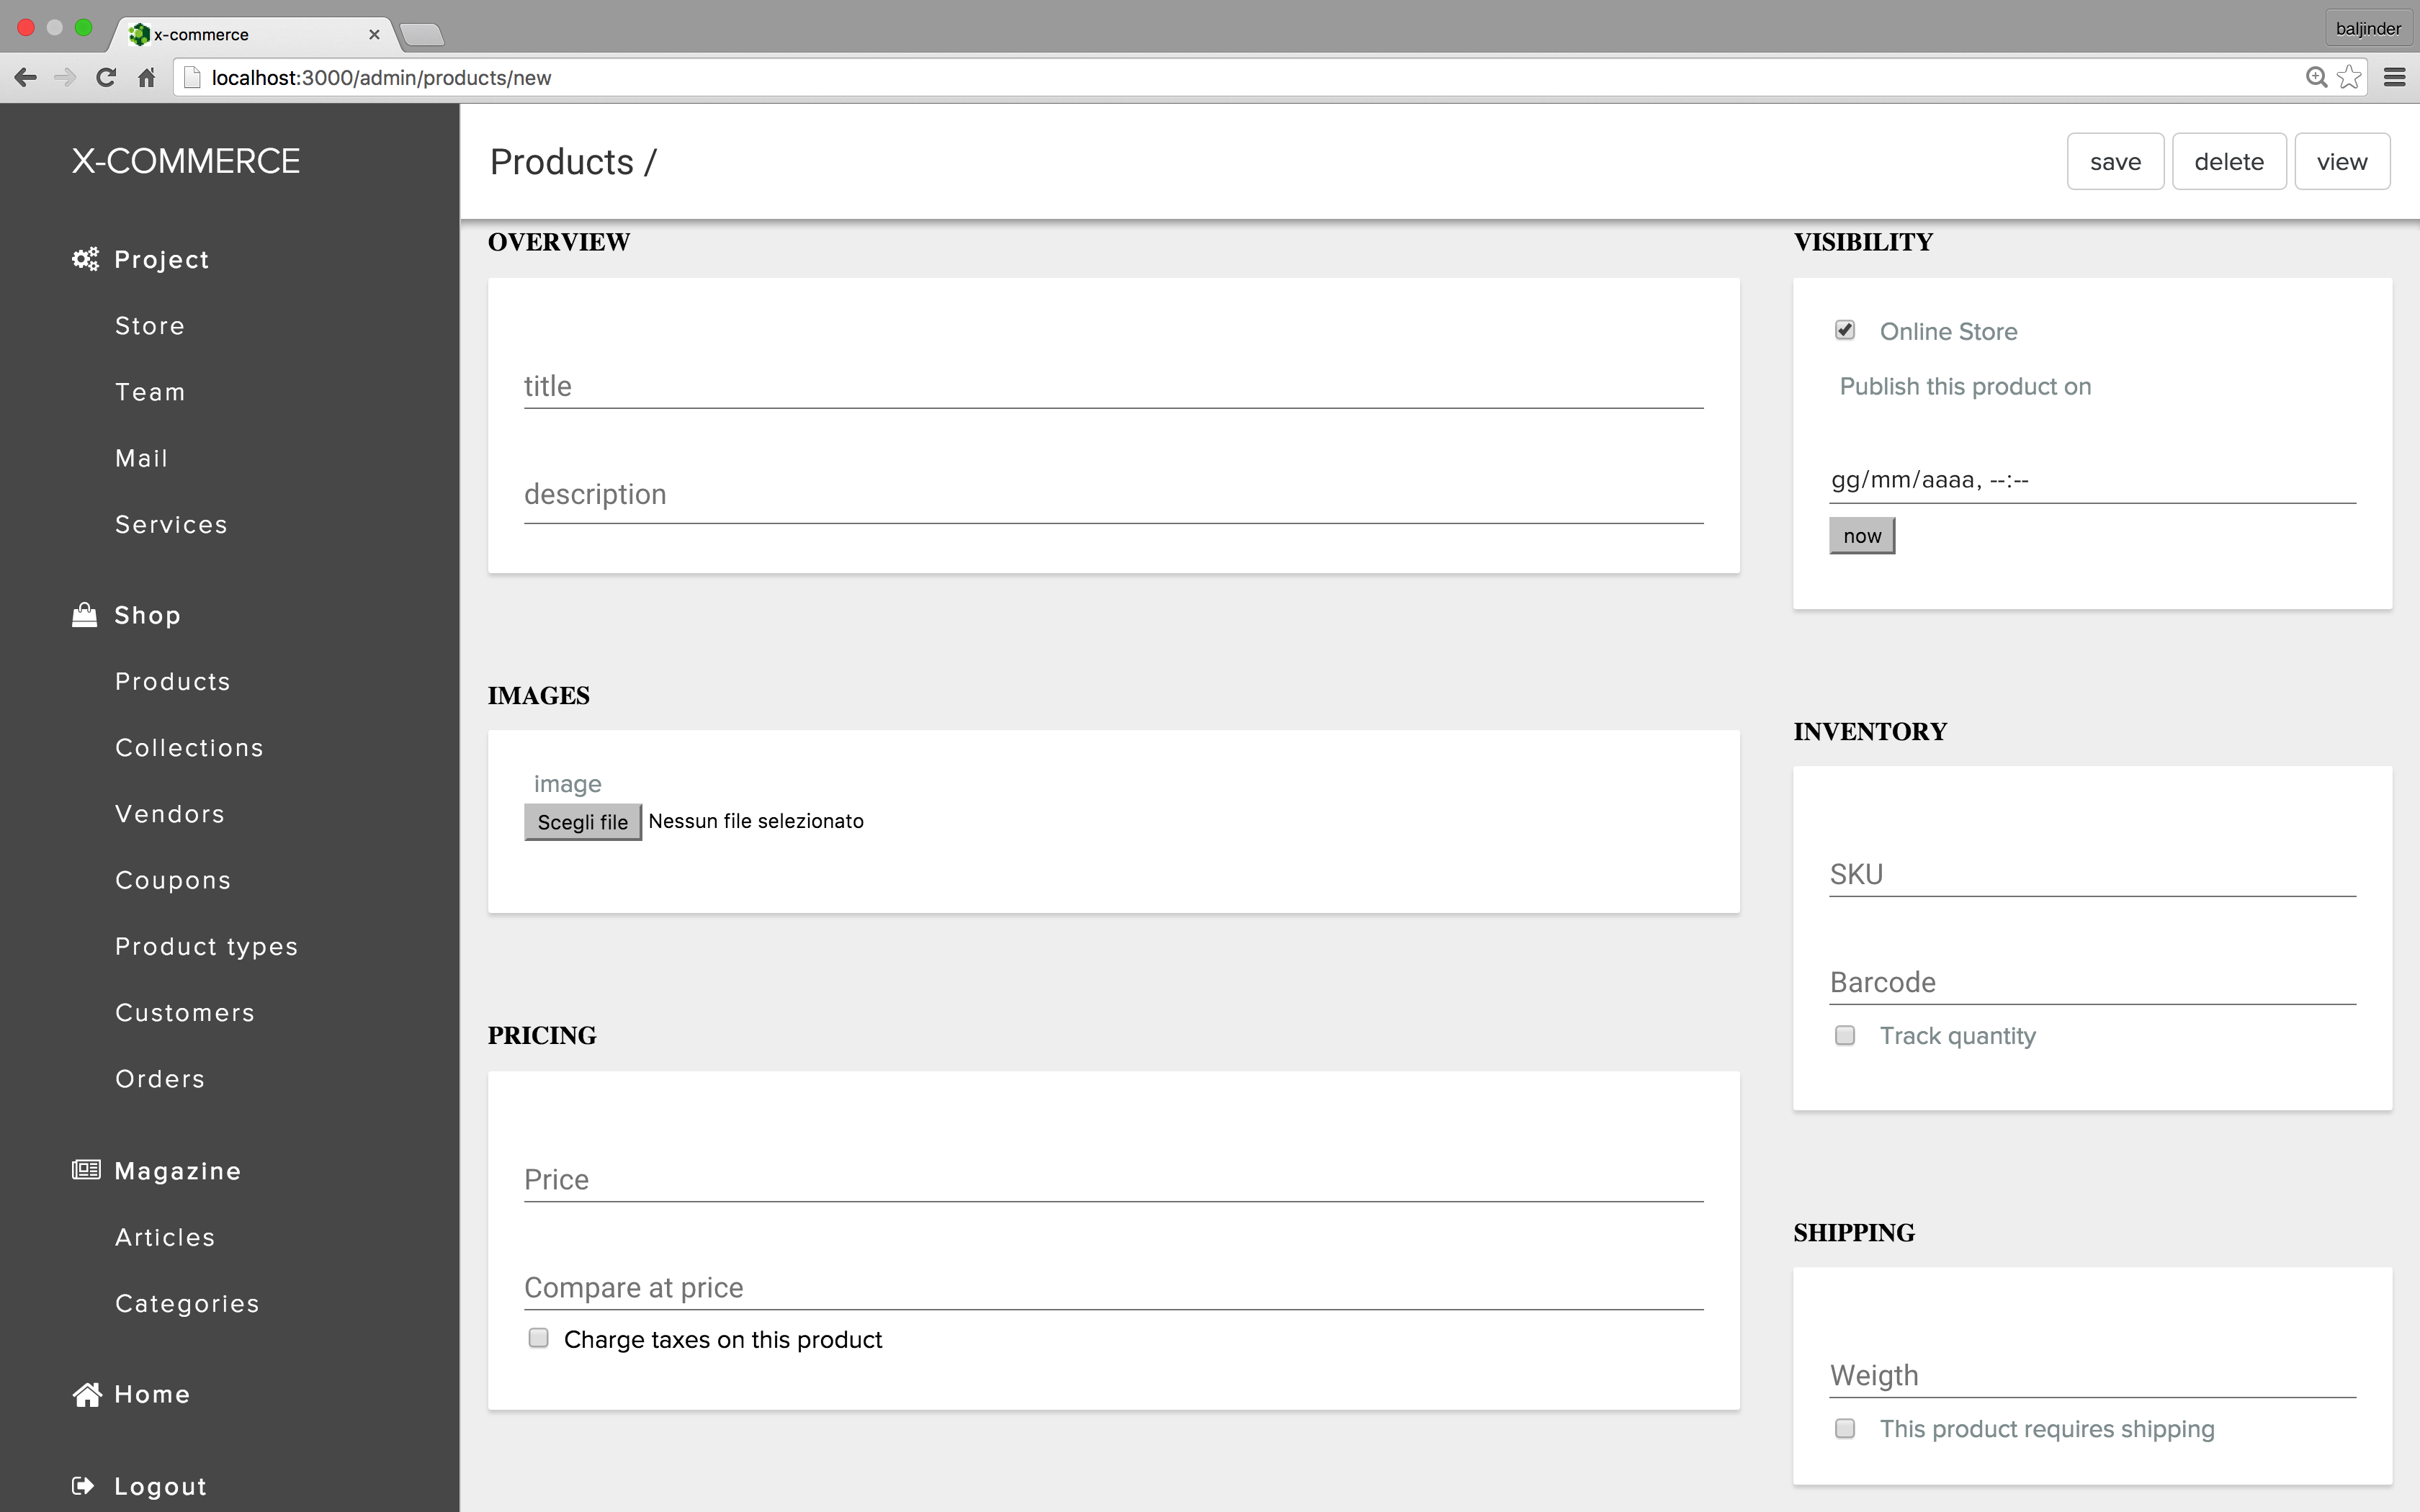
\includegraphics[width=1.0\linewidth]{images/chapter4/product-page-ex1.png}\hfill
\caption[page product first part form]{Page product example - first part form interface}
\label{fig:design_page}
\end{figure}
\newline
This first part of the page product consists of several components:
\begin{itemize}
\item
\begin{lstlisting}[language=html]
<part-product-header></part-product-header>
\end{lstlisting}
this component is used to represent the \emph{breadcrumb} and buttons to perform the action on the product;
\item
\begin{lstlisting}[language=html]
<part-product-info></part-product-info>
\end{lstlisting}
this element manages information based on a product such as the name and description;
\item
\begin{lstlisting}[language=html]
<part-product-visibility></part-product-visibility>
\end{lstlisting}
this component serves to schedule the date of publication of the product on the store;
\item
\begin{lstlisting}[language=html]
<part-product-image></part-product-image>
\end{lstlisting}
this component is used to represent the image of the product;
\end{itemize}
%second part of page product%
Following is shown a second part of the page product:
\begin{figure}[htb]
\centering
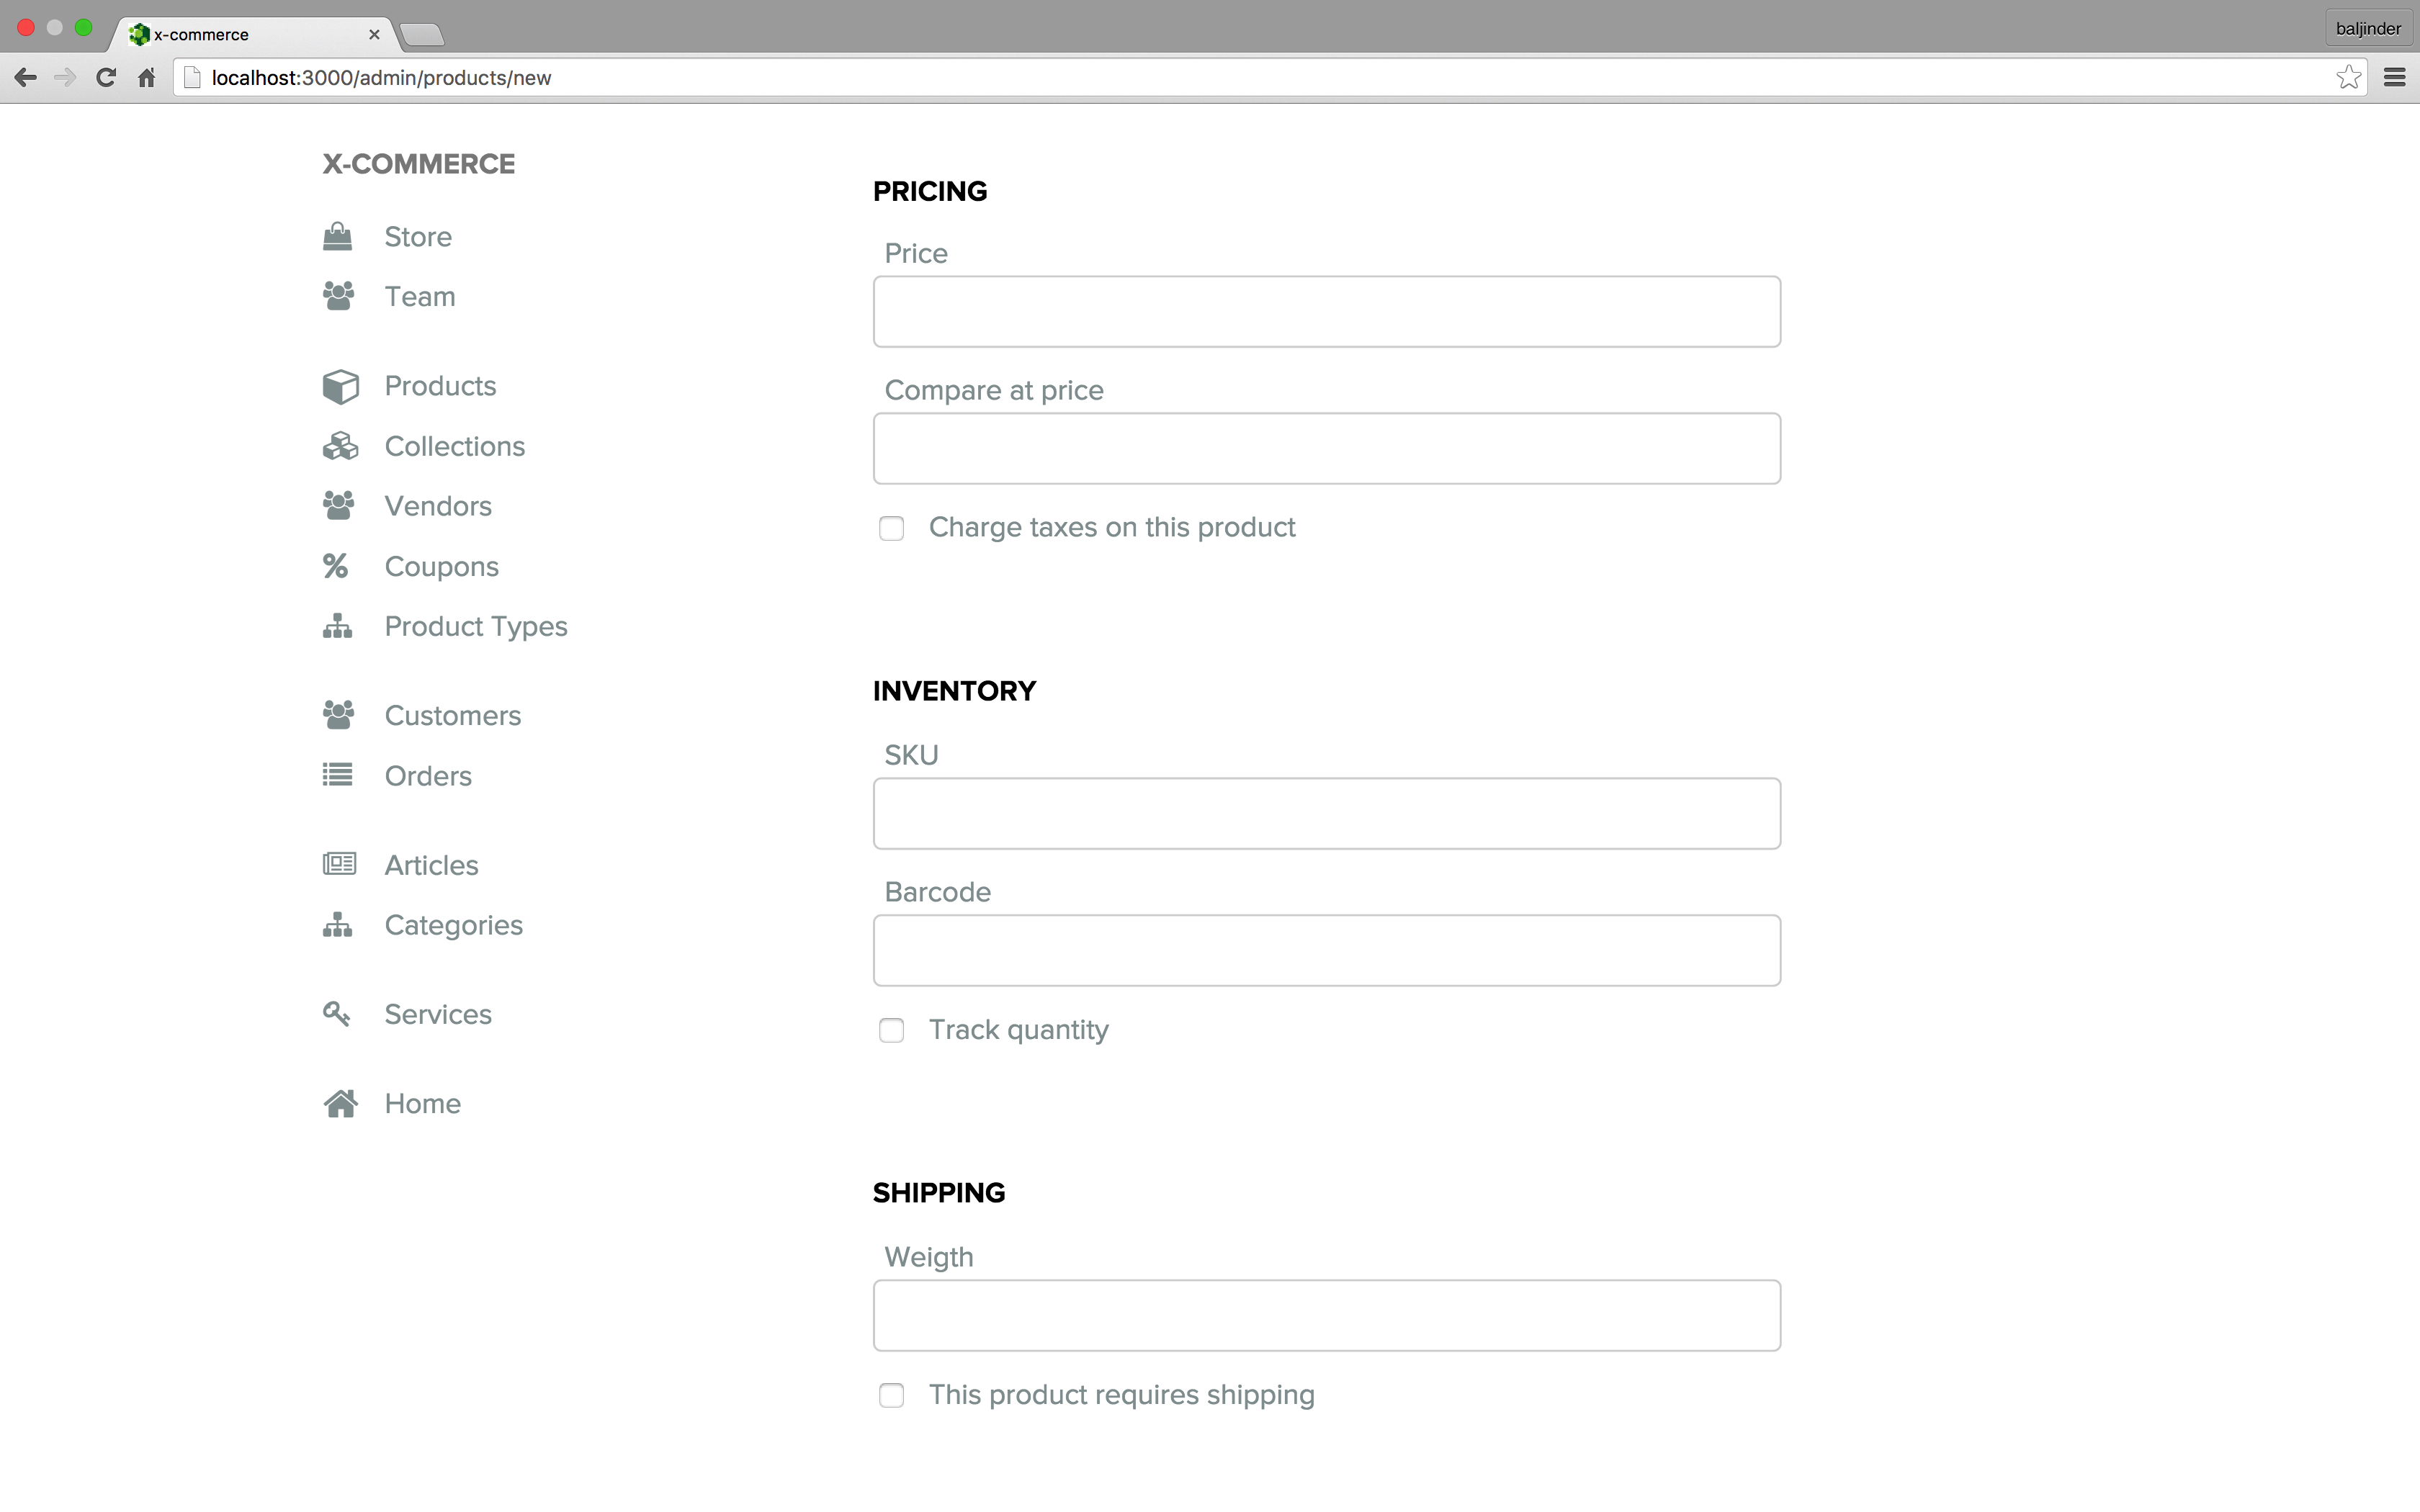
\includegraphics[width=0.9\linewidth]{images/chapter4/product-page-ex2.png}\hfill
\caption[page product second part form]{Page product example - second part form interface}
\label{fig:design_page}
\end{figure}
\newline
This second part of the page product contains other components:
\begin{itemize}
\item
\begin{lstlisting}[language=html]
<part-product-pricing></part-product-pricing>
\end{lstlisting}
this component represents the information relating to the price;
\item
\begin{lstlisting}[language=html]
<part-product-inventory></part-product-inventory>
\end{lstlisting}
this component is used to represents the information relating inventory as barcode and SKU( stock keeping unit);
\item
\begin{lstlisting}[language=html]
<part-product-shipping></part-product-shipping>
\end{lstlisting}
this component is used to represents the weigth of product;
\end{itemize}
%third part of page product%
Following is shown a third part of the page product:
\begin{figure}[htb]
\centering
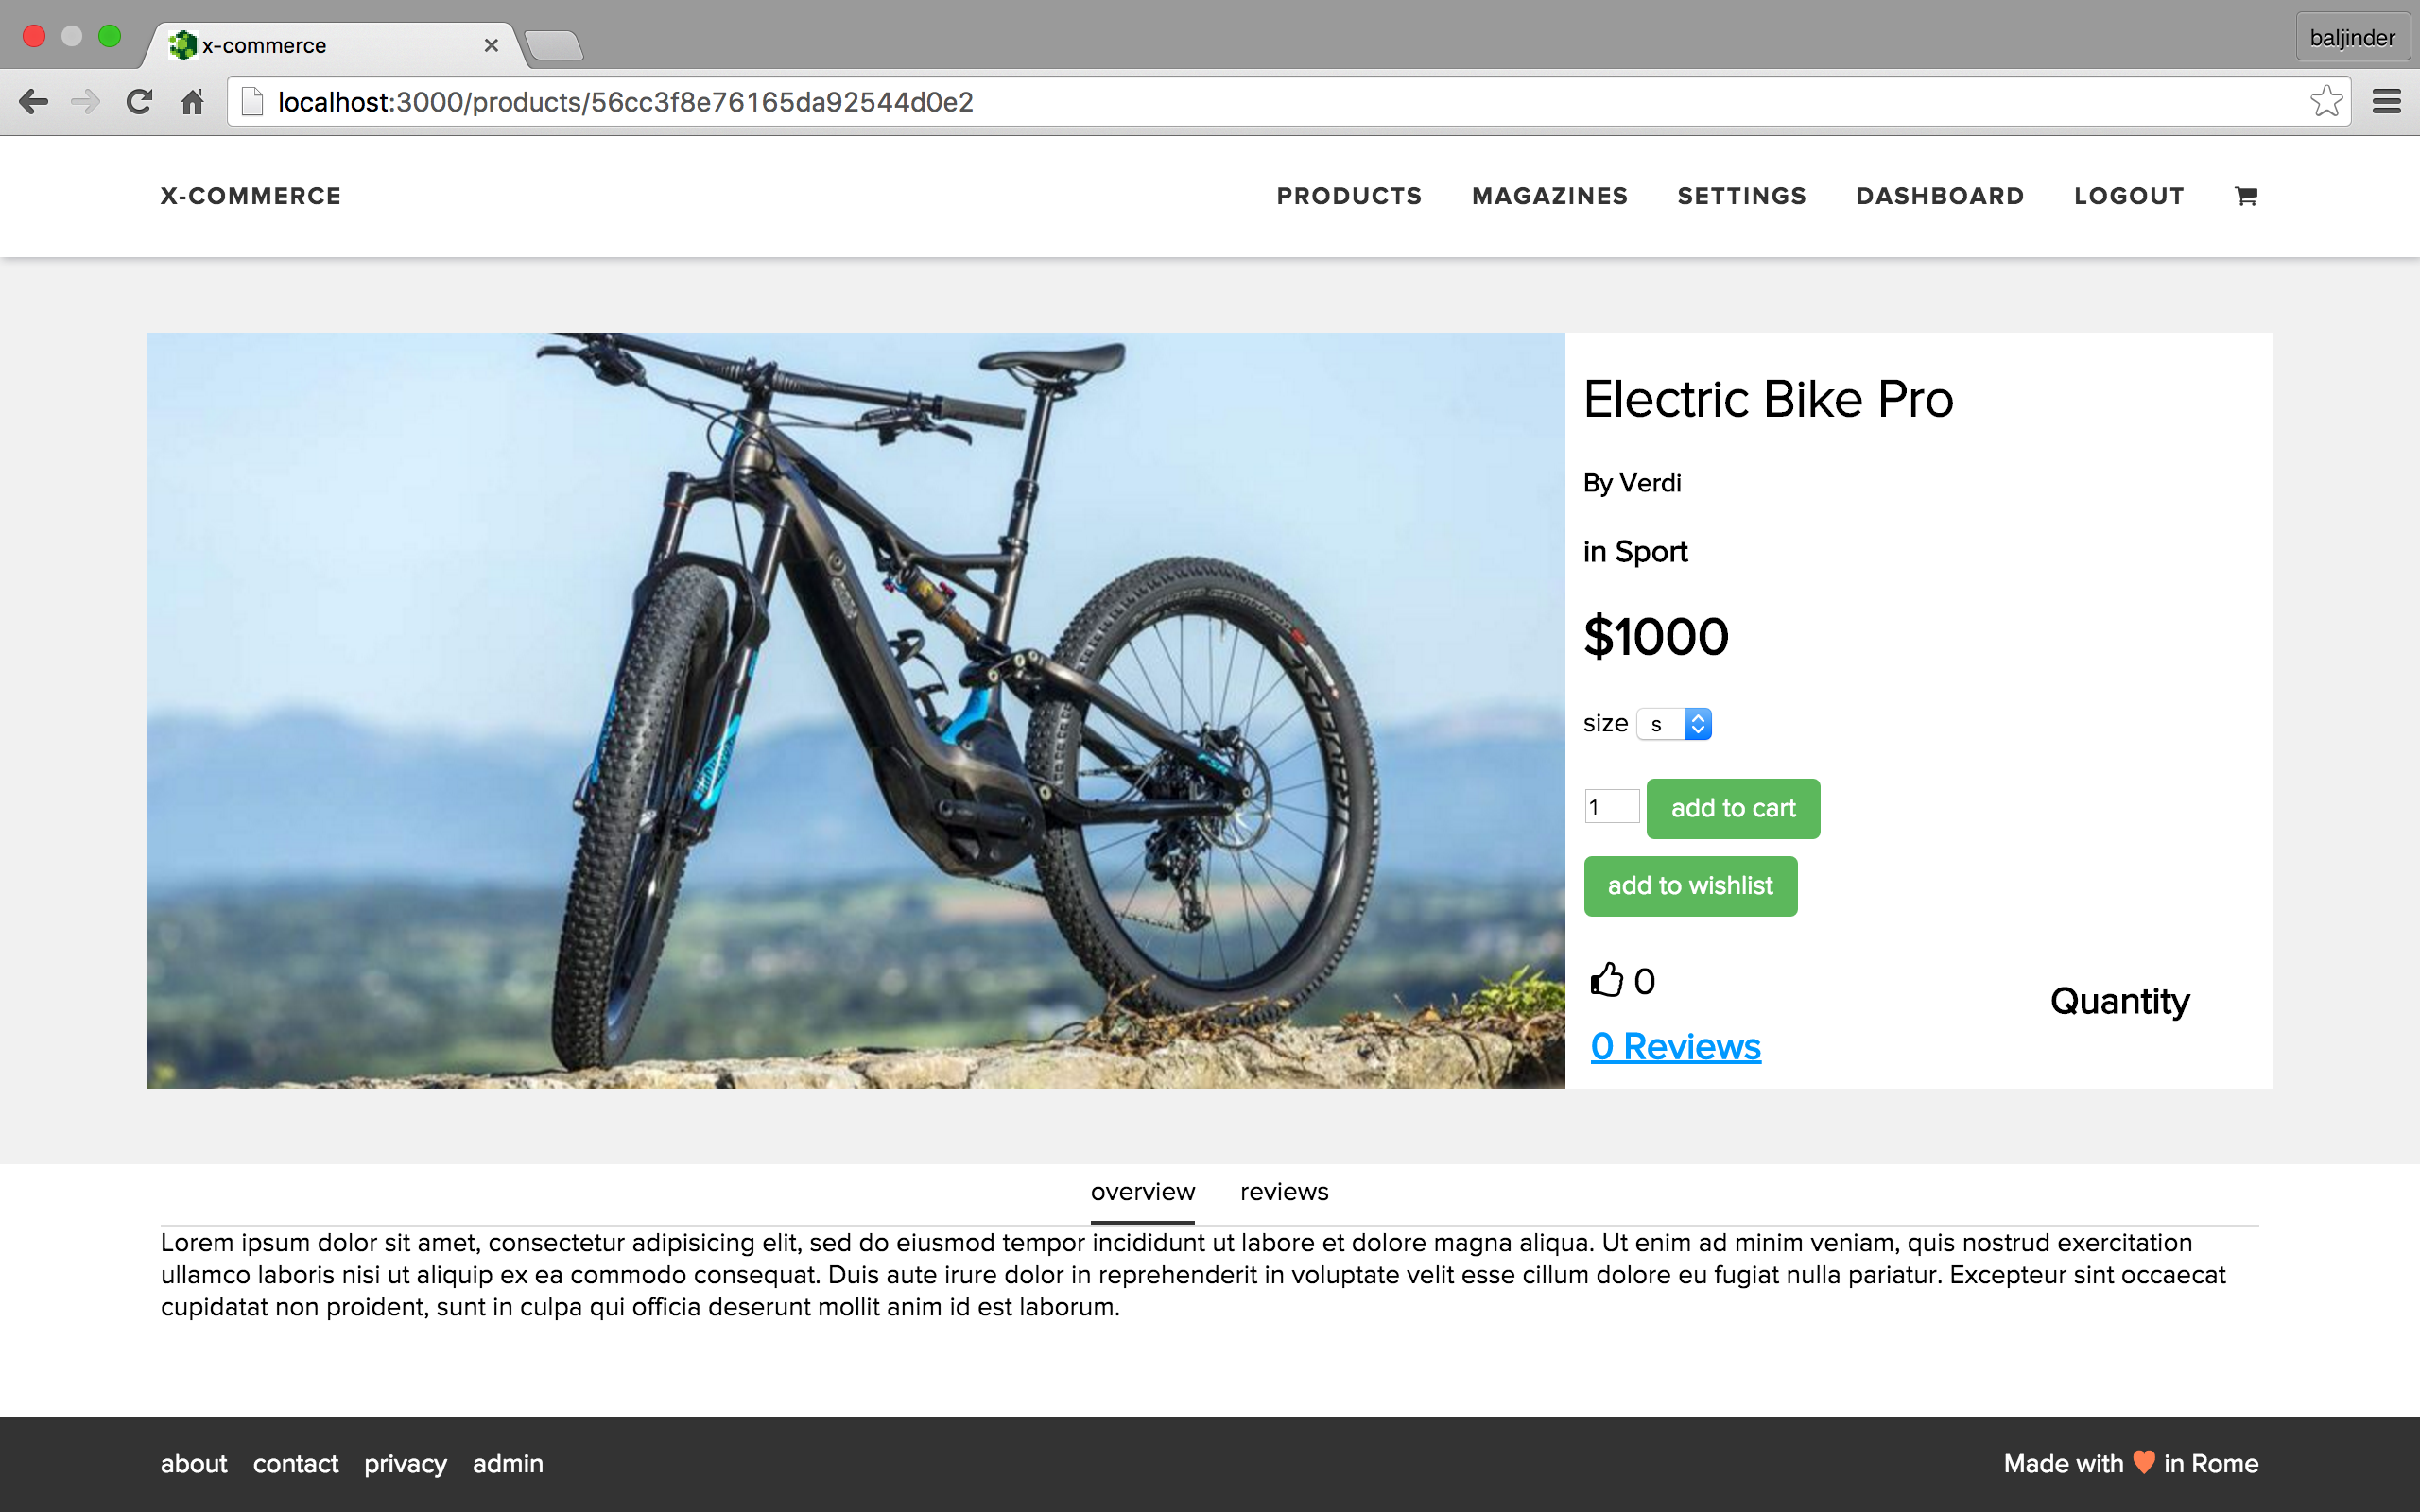
\includegraphics[width=1.0\linewidth]{images/chapter4/product-page-ex3.png}\hfill
\caption[page product third part form]{Page product example - third part form interface}
\label{fig:design_page}
\end{figure}
\newline
This third part of the page product contains other components:
\begin{itemize}
\item
\begin{lstlisting}[language=html]
<part-product-organization></part-product-organization>
\end{lstlisting}
this component hides all the operating logic to assign the current product to a seller, to one or more collections, define the type of product. Finally, it is possible to assign the tag to the product;
\item
\begin{lstlisting}[language=html]
<part-product-variants></part-product-variants>
\end{lstlisting}
this component hides the entire operating logic to create variants of a product;
\item
\begin{lstlisting}[language=html]
<part-product-actions></part-product-actions>
\end{lstlisting}
This component is the buttons of saving a product and its display at the client side;
\end{itemize}
Putting together these small self-contained components, is designed the product page. Now let's see how it designed the product page at client-side.
\subsubsection{Client side}
\begin{figure}[htb]
\centering
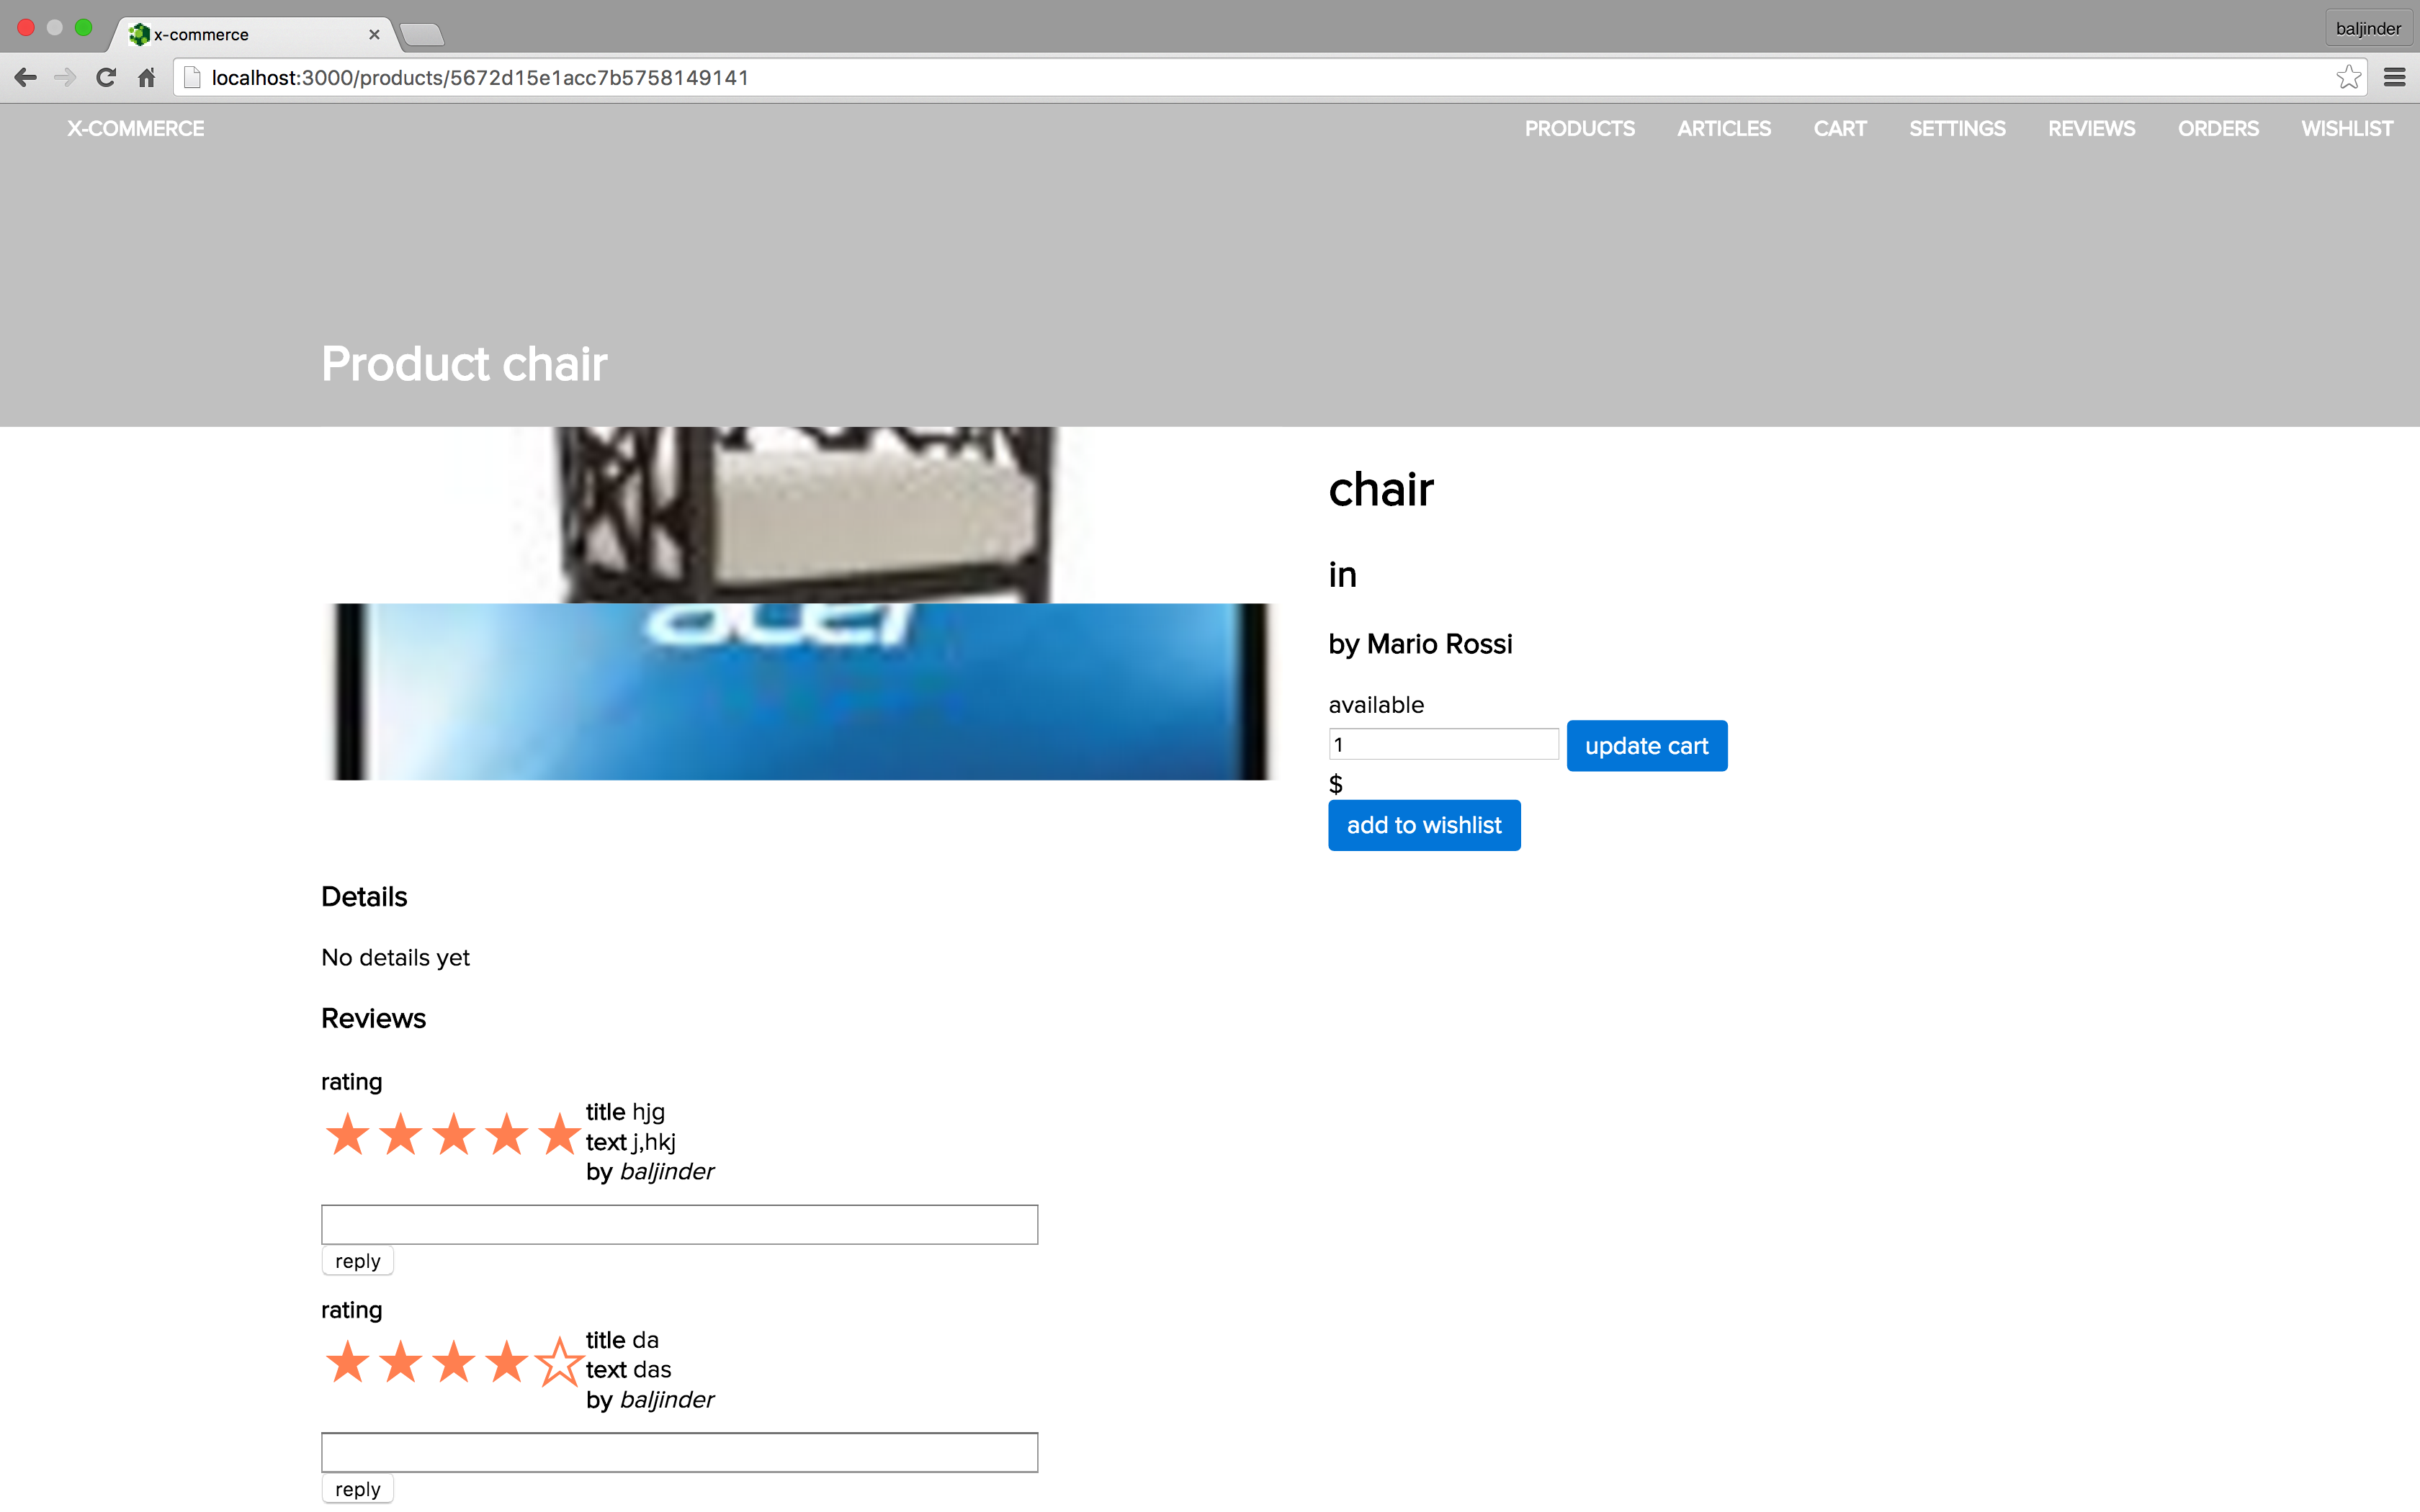
\includegraphics[width=0.9\linewidth]{images/chapter4/product-page-ex4.png}\hfill
\caption[page product client-side]{Page product client-side example}
\label{fig:design_page_prod_cli}
\end{figure}
The components making up the product page of the client are as follows:
\begin{lstlisting}[language=html]
<part-product-info></part-product-info>
<part-product-options></part-product-options>
<part-product-cart></part-product-cart>
<part-product-wish></part-product-wish>
<part-product-details></part-product-details>
<part-product-reviews></part-product-reviews>
\end{lstlisting}
It is evident the role of each component in the page.